\chapter{Proposta para análise de arquiteturas de microsserviços \ac{mmorpg}}
\label{cap3}

Para realizar a análise de consumo de recursos de uma arquitetura de jogos \ac{mmorpg} é necessário coletar / medir os recursos utilizados para posterior análise.
%
Na fase de coleta de informação, é possível utilizar ferramentas existentes para coletar informações sobre o consumo da rede (\textit{e.g.}, Tcpdump, Wireshark, etc.) e consumo de recursos computacionais do serviço (e.g., Golang Flame, Ruby Thread profiler tool, Golang profiler, \textit{etc.})
%
Estas ferramentas contribuem com a análise, sendo de extrema importância para a coleta de dados.



Contudo, se faz necessário uma arquitetura de microsserviços para jogos \ac{mmorpg} a fim de ser utilizado para análise.
%
Esta arquitetura será descrita na Seção~\ref{sec:arquitetura_proposta}.



\section{Arquitetura proposta para análise}
\label{sec:arquitetura_proposta}

Esta seção tem como objetivo descrever a arquitetura implementada para análise, baseada na arquitetura Salz~\cite{albion_online_unite}.
%
A mesma arquitetura é utilizada no jogo Sandbox-Interactive Albion\footnote{Sandbox-Interactive Albion: \url{https://albiononline.com/en/home}}.
%
Ela pode ser vista em uma visão macro na Figura~\ref{fig:salz}.


\begin{figure}[htb!]
\caption{Arquitetura de microsserviços proposta para análise.}
\label{fig:salz}
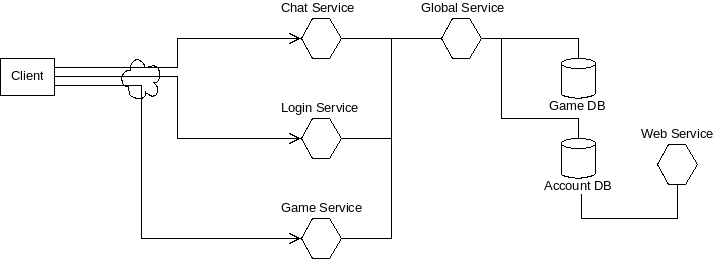
\includegraphics[height=5cm]{img/cap3/salz.png}
\centering

Adaptado de:~\cite{albion_online_unite}.
\end{figure}



Essa arquitetura contém os seguintes microsserviços:

\begin{itemize}
\item Login Service: Responsável por gerenciar as conexões do jogo e fornecer autorização aos clientes para os demais microsserviços.
  \item Chat Service: Receberá mensagens e distribuirá aos demais jogadores da mesma região ou enviará mensagens diretas a outros jogadores. Ele receberá a conexão diretamente do jogador, e por sua vez será necessário utilizar o \textit{Login Service} para autenticar a conexão.
  \item Game Service: Gerenciará um pedaço do ambiente do jogo. Cada microsserviço desta categoria será responsável por um pedaço do jogo, controlando as ações dos personagens em relação a sua área de interesse. Ele receberá a conexão diretamente do cliente, e por sua vez precisa utilizar o \textit{Login Service} para autenticar a conexão.
  \item Global Service: Este microsserviço resolve as requisições globais requisitadas pelo \textit{chat service}, \textit{login service} ou \textit{game service}.
  \item Web Service: Servirá para gerência de contas pessoais, autenticação e afins.
  \item Game DB: Banco de dados em memória utilizado pelos microsserviços.
  \item Account DB: Banco de dados persistente.
\end{itemize}


Para melhor compreendimento se faz necessário a descrição específica de funcionamento em cada microsserviço, tecnologias e protocolos utilizados e esquema de funcionamento.
%
Além disso será obrigatório descrever os microsserviços de GameDB e AccountDB utilizados na arquitetura.

\subsection{Login Service}

\subsection{Chat Service}

\subsection{Game Service}

\subsection{Global Service}

\subsection{Web Service}

\subsection{GameDB}

\subsection{AccountDB}

